\documentclass[a4paper, 12pt]{article}

% packages
\usepackage{amssymb}
\usepackage[fleqn]{mathtools}
\usepackage{tikz}
\usepackage{enumerate}
\usepackage{bussproofs}
\usepackage{xcolor}
\usepackage[margin=1.3cm]{geometry}
\usepackage{logicproof}
\usepackage{diagbox}
\usepackage{listings}
\usepackage{graphicx}
\usepackage{lstautogobble}
\usepackage{hyperref}
\usepackage{multirow}
\usepackage{tipa}
\usepackage{pgfplots}
\usepackage{adjustbox}

% tikz libraries
\usetikzlibrary{
    decorations.pathreplacing,
    arrows,
    shapes,
    shapes.gates.logic.US,
    circuits.logic.US,
    calc,
    automata,
    positioning,
    intersections
}

\pgfplotsset{compat=1.16}

\pgfmathdeclarefunction{gauss}{2}{%
  \pgfmathparse{1/(#2*sqrt(2*pi))*exp(-((x-#1)^2)/(2*#2^2))}%
}

\allowdisplaybreaks % allow environments to break
\setlength\parindent{0pt} % no indent

% shorthand for verbatim
% this clashes with logicproof, so maybe fix this at some point?
\catcode`~=\active
\def~#1~{\texttt{#1}}

% code listing
\lstdefinestyle{main}{
    numberstyle=\tiny,
    breaklines=true,
    showspaces=false,
    showstringspaces=false,
    tabsize=2,
    numbers=left,
    basicstyle=\ttfamily,
    columns=fixed,
    fontadjust=true,
    basewidth=0.5em,
    autogobble,
    xleftmargin=3.0ex,
    mathescape=true
}
\newcommand{\dollar}{\mbox{\textdollar}} %
\lstset{style=main}

% augmented matrix
\makeatletter
\renewcommand*\env@matrix[1][*\c@MaxMatrixCols c]{%
\hskip -\arraycolsep
\let\@ifnextchar\new@ifnextchar
\array{#1}}
\makeatother

% ceiling / floor
\DeclarePairedDelimiter{\ceil}{\lceil}{\rceil}
\DeclarePairedDelimiter{\floor}{\lfloor}{\rfloor}

% custom commands
\newcommand{\indefint}[2]{\int #1 \, \mathrm{d}#2}
\newcommand{\defint}[4]{\int_{#1}^{#2} #3 \, \mathrm{d}#4}
\newcommand{\pdif}[2]{\frac{\partial #1}{\partial #2}}
\newcommand{\dif}[2]{\frac{\mathrm{d}#1}{\mathrm{d}#2}}
\newcommand{\limit}[2]{\raisebox{0.5ex}{\scalebox{0.8}{$\displaystyle{\lim_{#1 \to #2}}$}}}
\newcommand{\limitsup}[2]{\raisebox{0.5ex}{\scalebox{0.8}{$\displaystyle{\limsup_{#1 \to #2}}$}}}
\newcommand{\summation}[2]{\sum\limits_{#1}^{#2}}
\newcommand{\product}[2]{\prod\limits_{#1}^{#2}}
\newcommand{\intbracket}[3]{\left[#3\right]_{#1}^{#2}}
\newcommand{\laplace}{\mathcal{L}}
\newcommand{\fourier}{\mathcal{F}}
\newcommand{\mat}[1]{\boldsymbol{#1}}
\renewcommand{\vec}[1]{\boldsymbol{#1}}
\newcommand{\rowt}[1]{\begin{bmatrix}
    #1
\end{bmatrix}^\top}
\DeclareMathOperator*{\argmax}{argmax}
\DeclareMathOperator*{\argmin}{argmin}

\newcommand{\lto}[0]{\leadsto\ }

\newcommand{\ulsmash}[1]{\underline{\smash{#1}}}

\newcommand{\powerset}[0]{\wp}
\renewcommand{\emptyset}[0]{\varnothing}

\makeatletter
\newsavebox{\@brx}
\newcommand{\llangle}[1][]{\savebox{\@brx}{\(\m@th{#1\langle}\)}%
  \mathopen{\copy\@brx\kern-0.5\wd\@brx\usebox{\@brx}}}
\newcommand{\rrangle}[1][]{\savebox{\@brx}{\(\m@th{#1\rangle}\)}%
  \mathclose{\copy\@brx\kern-0.5\wd\@brx\usebox{\@brx}}}
\makeatother
\newcommand{\lla}{\llangle}
\newcommand{\rra}{\rrangle}
\newcommand{\la}{\langle}
\newcommand{\ra}{\rangle}
\newcommand{\crnr}[1]{\text{\textopencorner} #1 \text{\textcorner}}
\newcommand{\bnfsep}[0]{\ |\ }
\newcommand{\concsep}[0]{\ ||\ }

\newcommand{\axiom}[1]{\AxiomC{#1}}
\newcommand{\unary}[1]{\UnaryInfC{#1}}
\newcommand{\binary}[1]{\BinaryInfC{#1}}
\newcommand{\trinary}[1]{\TrinaryInfC{#1}}
\newcommand{\quaternary}[1]{\QuaternaryInfC{#1}}
\newcommand{\quinary}[1]{\QuinaryInfC{#1}}
\newcommand{\dproof}[0]{\DisplayProof}
\newcommand{\llabel}[1]{\LeftLabel{\scriptsize #1}}
\newcommand{\rlabel}[1]{\RightLabel{\scriptsize #1}}

\newcommand{\ttbs}{\char`\\}
\newcommand{\lrbt}[0]{\ \bullet\ }

% colours
\newcommand{\violet}[1]{\textcolor{violet}{#1}}
\newcommand{\blue}[1]{\textcolor{blue}{#1}}
\newcommand{\red}[1]{\textcolor{red}{#1}}
\newcommand{\teal}[1]{\textcolor{teal}{#1}}

% reasoning proofs
\usepackage{ltablex}
\usepackage{environ}
\keepXColumns
\NewEnviron{reasoning}{
    \begin{tabularx}{\textwidth}{rlX}
        \BODY
    \end{tabularx}
}
\newcommand{\proofline}[3]{$(#1)$ & $#2$ & \hfill #3 \smallskip \\}
\newcommand{\proofarbitrary}[1]{& take arbitrary $#1$ \smallskip \\}
\newcommand{\prooftext}[1]{\multicolumn{3}{l}{#1} \smallskip \\}
\newcommand{\proofmath}[3]{$#1$ & = $#2$ & \hfill #3 \smallskip \\}
\newcommand{\prooftherefore}[1]{& $\therefore #1$ \smallskip \\}
\newcommand{\proofbc}[0]{\prooftext{\textbf{Base Case}}}
\newcommand{\proofis}[0]{\prooftext{\textbf{Inductive Step}}}

% ER diagrams
\newcommand{\nattribute}[4]{
    \node[draw, state, inner sep=0cm, minimum size=0.2cm, label=#3:{#4}] (#1) at (#2) {};
}
\newcommand{\mattribute}[4]{
    \node[draw, state, accepting, inner sep=0cm, minimum size=0.2cm, label=#3:{#4}] (#1) at (#2) {};
}
\newcommand{\dattribute}[4]{
    \node[draw, state, dashed, inner sep=0cm, minimum size=0.2cm, label=#3:{#4}] (#1) at (#2) {};
}
\newcommand{\entity}[3]{
    \node[] (#1-c) at (#2) {#3};
    \node[inner sep=0cm] (#1-l) at ($(#1-c) + (-1, 0)$) {};
    \node[inner sep=0cm] (#1-r) at ($(#1-c) + (1, 0)$) {};
    \node[inner sep=0cm] (#1-u) at ($(#1-c) + (0, 0.5)$) {};
    \node[inner sep=0cm] (#1-d) at ($(#1-c) + (0, -0.5)$) {};
    \draw
    ($(#1-c) + (-1, 0.5)$) -- ($(#1-c) + (1, 0.5)$) -- ($(#1-c) + (1, -0.5)$) -- ($(#1-c) + (-1, -0.5)$) -- cycle;
}
\newcommand{\relationship}[3]{
    \node[] (#1-c) at (#2) {#3};
    \node[inner sep=0cm] (#1-l) at ($(#1-c) + (-1, 0)$) {};
    \node[inner sep=0cm] (#1-r) at ($(#1-c) + (1, 0)$) {};
    \node[inner sep=0cm] (#1-u) at ($(#1-c) + (0, 1)$) {};
    \node[inner sep=0cm] (#1-d) at ($(#1-c) + (0, -1)$) {};
    \draw
    ($(#1-c) + (-1, 0)$) -- ($(#1-c) + (0, 1)$) -- ($(#1-c) + (1, 0)$) -- ($(#1-c) + (0, -1)$) -- cycle;
}

% AVL Trees
\newcommand{\avltri}[4]{
    \draw ($(#1)$) -- ($(#1) + #4*(0.5, -1)$) -- ($(#1) + #4*(-0.5, -1)$) -- cycle;
    \node at ($(#1) + #4*(0, -1) + (0, 0.5)$) {#3};
    \node at ($(#1) + #4*(0, -1) + (0, -0.5)$) {#2};
}

% RB Trees
\tikzset{rbtr/.style={inner sep=2pt, circle, draw=black, fill=red}}
\tikzset{rbtb/.style={inner sep=2pt, circle, draw=black, fill=black}}

% Samples
\tikzset{spos/.style={inner sep=2pt, circle, draw=black, fill=blue!20}}
\tikzset{sneg/.style={inner sep=2pt, circle, draw=black, fill=red!20}}

% Joins
\newcommand\ljoin{\stackrel{\mathclap{\normalfont\mbox{\tiny L}}}{\bowtie}}
\newcommand\rjoin{\stackrel{\mathclap{\normalfont\mbox{\tiny R}}}{\bowtie}}
\newcommand\ojoin{\stackrel{\mathclap{\normalfont\mbox{\tiny O}}}{\bowtie}}

\setcounter{MaxMatrixCols}{100}

% actual document
\begin{document}
    {\sc Computing $3^\text{rd}$ Year Notes} \hfill ~https://github.com/lin-e/imperial-revision~
    \rule{\textwidth}{0.1pt}
    \section*{CO317 - Graphics \hfill (60005)}
        \subsection*{Lecture 1 - Projections and Transformations}
            \subsubsection*{Two Dimensional Graphics}
                At the lowest level, in every operating system, graphics processing operates on the pixels in a window with primitives, such as;
                \begin{itemize}
                    \itemsep0em
                    \item ~SetPixel(int x, int y, int colour);~
                    \item ~DrawLine(int xs, int ys, int xf, int yf);~
                \end{itemize}
                However, we'd like to be able to draw scenes from a three-dimensional world and have it appear in two-dimensional graphics primitives.
            \subsubsection*{World Coordinate System}
                In order to achieve independence when drawing objects, we define a world coordinate system.
                For example, let our world be defined in meters, we can then allow a pixel to represent a millimetre.
                A viewing area is a window, and is defined as part of our 3D world.
                \textbf{Clipping} occurs when we attempt to draw outside (dashed) of the \violet{window};
                \begin{lstlisting}
                    SetWindow(30, 10, 70, 50)
                    DrawLine(40, 3, 90, 30)
                    DrawLine(50, 60, 60, 40)
                \end{lstlisting}
                \begin{center}
                    \begin{tikzpicture}[x=0.075cm, y=0.075cm]
                        \draw (0, 0) edge[->] (0, 55);
                        \draw (0, 0) edge[->] (75, 0);

                        \draw[violet] (30, 10) -- (30, 50) -- (70, 50) -- (70, 10) -- cycle;
                        \draw[dashed]
                        (0, 10) -- (30, 10)
                        (0, 50) -- (30, 50)
                        (30, 0) -- (30, 10)
                        (70, 0) -- (70, 10);

                        \draw[dashed]
                        (40, 3) -- (52.963, 10)
                        (70, 19.2) -- (90, 30);
                        \draw (52.963, 10) -- (70, 19.2);

                        \draw[dashed] (50, 60) -- (55, 50);
                        \draw (55, 50) -- (60, 40);

                        \node at (-10, 10) {10};
                        \node at (-10, 50) {50};
                        \node at (30, -10) {30};
                        \node at (70, -10) {70};
                    \end{tikzpicture}
                \end{center}
                However, this isn't as trivial to do in 3D, as it cannot simply be left to the operating system.
                While we can represent 3D objects as a series of 2D commands, it's inefficient and expensive for the OS to perform the clipping (therefore we should do this manually).
            \subsubsection*{Normalisation}
                A normalisation process is required to convert from device independent commands (where screen resolution isn't taken into account) to drawing commands using pixels.
                Consider a point in the world coordinate window $(X_w, Y_w)$, and its corresponding result on the viewport (pixel coordinates; $(X_v, Y_v)$);
                \begin{center}
                    \begin{tikzpicture}[x=0.66cm, y=0.66cm]
                        \draw[rounded corners] (0, 0) -- (16, 0) -- (16, 9) -- (0, 9) -- cycle;

                        \draw (2, 2) -- (6, 2) -- (6, 6) -- (2, 6) -- cycle;
                        \node[rbtb] at (3, 3.5) {};
                        \node at (4, 4) {$(X_v, Y_v)$};

                        \begin{scope}[shift={(-9, 3)}]
                            \draw (0, 0) -- (6, 0) -- (6, 6) -- (0, 6) -- cycle;
                            \node[rbtb] at (1.5, 2.25) {};
                            \node at (2.5, 2.75) {$(X_w, Y_w)$};
                        \end{scope}

                        \draw[dashed]
                        (-9, 3) -- (2, 2)
                        (-3, 3) -- (6, 2)
                        (-3, 9) -- (6, 6)
                        (-9, 9) -- (2, 6)
                        (-9, 3) -- (-9, 0)
                        (-3, 3) -- (-3, 0)
                        (2, 2) -- (2, 0)
                        (6, 2) -- (6, 0);

                        \node at (-9, -1) {$W_{xmin}$};
                        \node at (-3, -1) {$W_{xmax}$};
                        \node at (2, -1) {$V_{xmin}$};
                        \node at (6, -1) {$V_{xmax}$};
                    \end{tikzpicture}
                \end{center}
                The expressions are similar for $Y$;
                $$\frac{(X_w - W_{xmin})}{(W_{xmax} - W_{xmin})} = \frac{(X_v - V_{xmin})}{(V_{xmax} - V_{xmin})} \Rightarrow X_v = \frac{(X_w - W_{xmin})(V_{xmax} - V_{xmin})}{(W_{xmax} - W_{xmin})} + V_{xmin}$$
                This gives us the resulting pair of linear equations (intuitively), where the constants found from the known values $W_{xmin}, V_{xmax}$, etc. are used to define the normalisation;
                \begin{align*}
                    X_v & = AX_w + B \\
                    Y_v & = CY_w + D
                \end{align*}
            \subsubsection*{Polygon Rendering}
                Most graphics applications deal with very simple objects - flat / planar polyhedra, referred to as \textbf{faces} or \textbf{facets}.
                These are graphic primitives, and can be used to approximate any shape.
                Consider the following tetrahedron, consisting of four vertices;
                \begin{center}
                    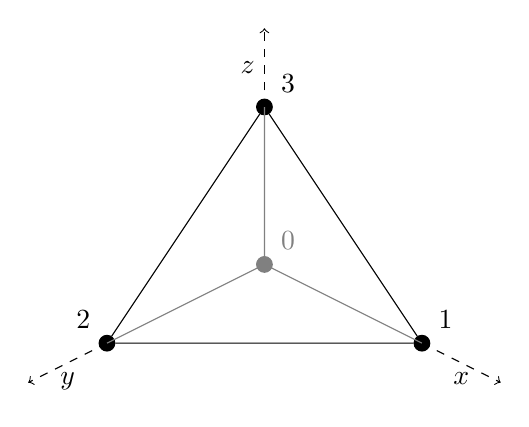
\begin{tikzpicture}
                        \node[inner sep=2pt, circle, draw=black!50, fill=black!50] at (0, 0) {};
                        \node[rbtb] (n3) at (0, 2) {};
                        \node[rbtb] (n1) at (2, -1) {};
                        \node[rbtb] (n2) at (-2, -1) {};

                        \node[black!50] at (0.3, 0.3) {0};
                        \node at (0.3, 2.3) {3};
                        \node at (2.3, -0.7) {1};
                        \node at (-2.3, -0.7) {2};

                        \draw[black!50]
                        (0, 0) -- (0, 2)
                        (0, 0) -- (2, -1)
                        (0, 0) -- (-2, -1);

                        \draw
                        (0, 2) edge[dashed, ->, left] node{$z$} (0, 3)
                        (2, -1) edge[dashed, ->, below] node{$x$} (3, -1.5)
                        (-2, -1) edge[dashed, ->, below] node{$y$} (-3, -1.5)
                        (n3) -- (n1) -- (n2) -- (n3);
                    \end{tikzpicture}
                \end{center}
                For this, we need a mixture of different data, including numerical data about the actual 3D coordinates of the vertices, as well as topological data regarding what vertices are connected to what.
                This can be represented in the following tables;
                \begin{center}
                    \hfill
                    \begin{tabular}{c|c}
                        \multicolumn{2}{c}{vertex data} \\
                        \hline
                        index & location \\
                        \hline
                        $0$ & $(0, 0, 0)$ \\
                        $1$ & $(1, 0, 0)$ \\
                        $2$ & $(0, 1, 0)$ \\
                        $3$ & $(0, 0, 1)$
                    \end{tabular}
                    \hfill
                    \begin{tabular}{c|c}
                        \multicolumn{2}{c}{face data} \\
                        \hline
                        index & vertices \\
                        \hline
                        $0$ & 0 1 3 \\
                        $1$ & 0 2 1 \\
                        $2$ & 0 3 2 \\
                        $3$ & 1 2 3
                    \end{tabular}
                    \hfill \phantom{}
                \end{center}
                This separation allows for the vertices to move without affecting the faces.
            \subsubsection*{Projections}
                In order to draw a 3D wire frame, the points must first be converted into a 2D representation, via a \textbf{projection}, which can then be drawn with simple drawing primitives.
                Intuitively, we have an observer (a focal point) where all viewing rays converge.
                The observer is located between a projection surface $P$ and an object $V$.
                While it's possible to project onto any surface, we only consider linear projections onto a flat surface.
            \subsubsection*{Orthographic Projections}
                The simplest form of a projection is an \textbf{orthographic projection}.
                The assumptions made are that the viewpoint is located at $z = -\infty$, and the plane of projection is $z = 0$.
                With the viewing point being infinitely far away, the rays become parallel.
                This gives all projectors the same direction;
                $$\vec{d} = \begin{bmatrix}
                    0 \\ 0 \\ -1
                \end{bmatrix}$$
                This gives the following, with each projection line having the equation $\vec{P} = \vec{V} + \mu \vec{d}$;
                \begin{center}
                    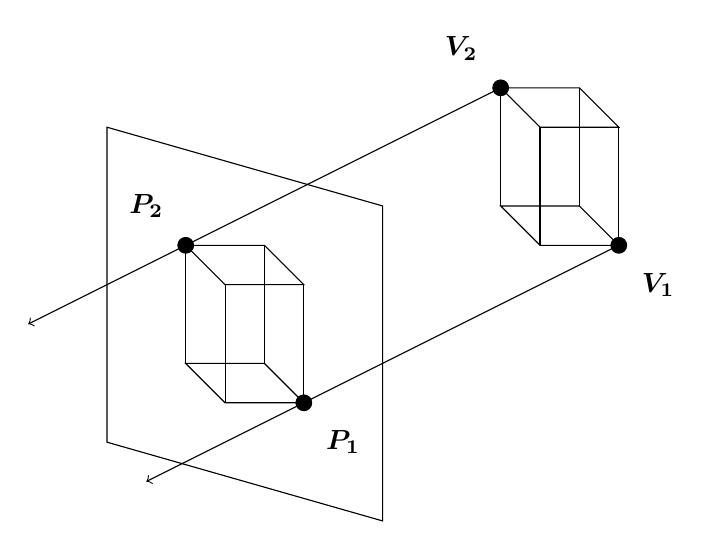
\begin{tikzpicture}
                        \draw (-1, 1.5) -- (2.5, 0.5) -- (2.5, -3.5) -- (-1, -2.5) -- cycle;
                        \begin{scope}[shift={(0, 0)}]
                            \draw (0, 0) -- (1, 0) -- (1.5, -0.5) -- (0.5, -0.5) -- cycle;
                            \draw (0, -1.5) -- (1, -1.5) -- (1.5, -2) -- (0.5, -2) -- cycle;
                            \draw
                            (0, 0) -- (0, -1.5)
                            (1, 0) -- (1, -1.5)
                            (1.5, -0.5) -- (1.5, -2)
                            (0.5, -0.5) -- (0.5, -2);
                        \end{scope}
                        \begin{scope}[shift={(4, 2)}]
                            \draw (0, 0) -- (1, 0) -- (1.5, -0.5) -- (0.5, -0.5) -- cycle;
                            \draw (0, -1.5) -- (1, -1.5) -- (1.5, -2) -- (0.5, -2) -- cycle;
                            \draw
                            (0, 0) -- (0, -1.5)
                            (1, 0) -- (1, -1.5)
                            (1.5, -0.5) -- (1.5, -2)
                            (0.5, -0.5) -- (0.5, -2);
                        \end{scope}

                        \draw
                        (4, 2) edge[->] (-2, -1)
                        (5.5, 0) edge[->] (-0.5, -3);

                        \node[rbtb] at (4, 2) {};
                        \node[rbtb] at (5.5, 0) {};
                        \node[rbtb] at (0, 0) {};
                        \node[rbtb] at (1.5, -2) {};

                        \node at (3.5, 2.5) {$\vec{V_2}$};
                        \node at (6, -0.5) {$\vec{V_1}$};
                        \node at (-0.5, 0.5) {$\vec{P_2}$};
                        \node at (2, -2.5) {$\vec{P_1}$};
                    \end{tikzpicture}
                \end{center}
                By substituting in the direction $\vec{d}$ we have determined, it gives the following Cartesian equations for each component;
                \begin{align*}
                    P_x & = V_x + 0 \\
                    P_y & = V_y + 0 \\
                    P_z & = V_z - \mu \\
                \end{align*}
                However, since we have the projection plane $z = 0$, we also know that $P_z = 0$, therefore we don't need to solve for $\mu$.
                From this, we can determine the projected location is the 3D $x$ and $y$ components of the vertex;
                $$\vec{P} = \begin{bmatrix}
                    V_x \\ V_y \\ 0
                \end{bmatrix}$$
                Viewing the wireframe for a cube directly from a face would look like the following;
                \begin{center}
                    \begin{tikzpicture}[x=1.5cm, y=1.5cm]
                        \draw (0, 0) -- (1, 0) -- (1, 1) -- (0, 1) -- cycle;
                    \end{tikzpicture}
                \end{center}
            \subsubsection*{Perspective Projection}
                While orthographic projections are fine when depth isn't a consideration (such as objects mostly being at the same distance from the viewer), it's insufficient for close work, where we want details to be realistic.
                The difference here is that we are no longer at an infinite distance (instead being at the origin), and the projection plane is $z = f$ (where $f$ stands for focal length);
                \begin{center}
                    \begin{tikzpicture}
                        \draw
                        (0, 0) edge[->] (10, 0)
                        (0, 0) edge[->] (0, 7);
                        \node at (-0.5, 7) {$y$};
                        \node at (10, -0.5) {$x$};
                        \node at (9, 4) {$z$};

                        \draw (2, 1) -- (2, 4) -- (6, 4) -- (6, 1) -- cycle;
                        \draw
                        (0, 0) -- (2, 1)
                        (2, 1) edge[dashed] (6, 3)
                        (6, 3) edge[->] (9, 4.5);

                        \draw (5, 7) -- (7, 6) -- (5.5, 5) -- cycle;
                        \node[rbtb] at (5, 7) {};
                        \node[rbtb] at (7, 6) {};
                        \node at (4.5, 7) {$\vec{V_1}$};
                        \node at (7.5, 6) {$\vec{V_2}$};

                        \draw (2.5, 3.5) -- (3.5, 3) -- (2.75, 2.5) -- cycle;
                        \node[rbtb] at (2.5, 3.5) {};
                        \node[rbtb] at (3.5, 3) {};
                        \node at (2, 3.5) {$\vec{P_1}$};
                        \node at (4, 3) {$\vec{P_2}$};

                        \draw[black!50]
                        (5, 7) -- (0, 0)
                        (7, 6) -- (0, 0);

                        \draw
                        (0, 0) edge[dashed] (0, -2)
                        (2, 1) edge[dashed] (2, -1)
                        (0, -1.5) edge[<->, below] node{$f$} (2, -0.5);
                    \end{tikzpicture}
                \end{center}
                This gives us the following equation (since all projectors must go through the origin);
                $$\vec{P} = \mu \vec{V}$$
                We can work out the value of $\mu$, let it be $\mu_p$ as follows;
                \begin{align*}
                    P_z & = f & \text{by projection plane} \\
                    \mu_p & = \frac{P_z}{V_z} \\
                    & = \frac{f}{V_z} \\
                    P_x & = \mu_p V_x \\
                    & = \frac{f V_x}{V_z} \\
                    P_y & = \mu_p V_y \\
                    & = \frac{f V_y}{V_z}
                \end{align*}
                Viewing the wireframe for a cube directly from a face would look like the following (note the difference to the orthographic projection);
                \begin{center}
                    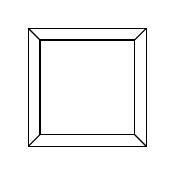
\begin{tikzpicture}[x=1.5cm, y=1.5cm]
                        \draw (0, 0) -- (1, 0) -- (1, 1) -- (0, 1) -- cycle;
                        \draw (0.1, 0.1) -- (0.9, 0.1) -- (0.9, 0.9) -- (0.1, 0.9) -- cycle;
                        \draw
                        (0, 0) -- (0.1, 0.1)
                        (1, 0) -- (0.9, 0.1)
                        (1, 1) -- (0.9, 0.9)
                        (0, 1) -- (0.1, 0.9);
                    \end{tikzpicture}
                \end{center}
            \subsubsection*{Transformations}
                Scenes are defined in a particular coordinate system, but we want to be able to draw a scene from any angle.
                To do so, it's easier to have the viewpoint at the origin, and the $z$-axis as the direction of view.
                As such, we need to be able to \textbf{transform} the coordinates of a scene.
                \begin{center}
                    \begin{tikzpicture}
                        \begin{scope}[shift={(0, 0)}]
                            \draw
                            (0, 0) edge[->, below] node{$x$} (5, 0)
                            (0, 0) edge[->, left] node{$y$} (0, 2)
                            (0, 0) edge[->, above] node{$z$} (2, 1);

                            \begin{scope}[shift={(2.5, 0.75)}]
                                \draw (0, 0) -- (1, 0) -- (1, 1) -- (0, 1) -- cycle;
                                \draw
                                (0, 0) -- (0.5, 0.5)
                                (1, 0) -- (1.5, 0.5)
                                (1, 1) -- (1.5, 1.5)
                                (0, 1) -- (0.5, 1.5);
                                \draw (0.5, 0.5) -- (1.5, 0.5) -- (1.5, 1.5) -- (0.5, 1.5) -- cycle;
                            \end{scope}

                            \draw
                            (0, 0) edge[dashed, ->, below] node{$C_x$} (4, 0)
                            (4, 0) edge[dashed, ->, right] node{\ \ $C_z$} (6, 1)
                            (6, 1) edge[dashed, ->, right] node{$C_y$} (6, 3)
                            (6, 3) edge[->, above] node{$\vec{d}$} (5, 2.5);

                            \node at (6.5, 3) {$\vec{C}$};
                            \node at (-0.5, 0) {$\vec{O}$};
                        \end{scope}
                        \begin{scope}[shift={(8, 0)}]
                            \draw
                            (0, 0) edge[dashed] (5, 0)
                            (0, 0) edge[dashed] (0, 2)
                            (0, 0) edge[dashed] (2, 1);

                            \begin{scope}[shift={(2.5, 0.75)}]
                                \draw (0, 0) -- (1, 0) -- (1, 1) -- (0, 1) -- cycle;
                                \draw
                                (0, 0) -- (0.5, 0.5)
                                (1, 0) -- (1.5, 0.5)
                                (1, 1) -- (1.5, 1.5)
                                (0, 1) -- (0.5, 1.5);
                                \draw (0.5, 0.5) -- (1.5, 0.5) -- (1.5, 1.5) -- (0.5, 1.5) -- cycle;
                            \end{scope}

                            \draw
                            (6, 3) edge[->, below] node{$z$} (5, 2.5)
                            (6, 3) edge[->, right] node{$y$} (5.5, 4)
                            (6, 3) edge[->, below] node{$x$} (5.25, 3.5);

                            \node at (6.5, 3) {$\vec{O}$};
                        \end{scope}
                    \end{tikzpicture}
                \end{center}
                These are done by the application of transformation matrices.
                For example, a standard transformation to make an object twice as big from the origin;
                $$\begin{bmatrix}
                    x^\prime \\ y^\prime \\ z^\prime
                \end{bmatrix} = \begin{bmatrix}
                    2 & 0 & 0 \\
                    0 & 2 & 0 \\
                    0 & 0 & 2
                \end{bmatrix} \begin{bmatrix}
                    x \\ y \\ z
                \end{bmatrix}$$
            \subsubsection*{Translation}
                However, being restricted to matrix operations with $\mathbb{R}^{3 \times 3}$ means that we cannot represent translations (for example, a shift of two units on the $x$-axis, such that $x^\prime = x + 2$).
                The solution to this is to use 4D \textbf{homogenous coordinates}, where we assume the fourth dimension is fixed to 1.
                $$\begin{bmatrix}
                    x^\prime \\ y^\prime \\ z^\prime \\ 1
                \end{bmatrix} = \begin{bmatrix}
                    1 & 0 & 0 & 2 \\
                    0 & 1 & 0 & 0 \\
                    0 & 0 & 1 & 0 \\
                    0 & 0 & 0 & 1
                \end{bmatrix} \begin{bmatrix}
                    x \\ y \\ z \\ 1
                \end{bmatrix}$$
                Frequently the last ordinate is 1, however in general it is a scale factor;
                $$\underbrace{(p_x, p_y, p_z, s)}_\text{homogeneous} \Leftrightarrow \underbrace{\left(\frac{p_x}{s}, \frac{p_y}{s}, \frac{p_z}{s}\right)}_\text{Cartesian}$$
            \subsubsection*{Affine Transformations}
                Affine transformations preserve parallel lines.
                Most of the transformations we require are affine, with the most important being scaling, rotation, and translation;
                \begin{itemize}
                    \itemsep0em
                    \item \textbf{scaling} \hfill by $(s_x, s_y, s_z)$
                        $$\begin{bmatrix}
                            s_x & 0 & 0 & 1 \\
                            0 & s_y & 0 & 1 \\
                            0 & 0 & s_z & 1 \\
                            0 & 0 & 0 & 1
                        \end{bmatrix} \begin{bmatrix}
                            p_x \\ p_y \\ p_z \\ 1
                        \end{bmatrix} = \begin{bmatrix}
                            s_x p_x \\
                            s_y p_y \\
                            s_z p_z \\
                            1
                        \end{bmatrix}$$
                    \item \textbf{rotation}
                        \smallskip

                        In order to define a rotation, we need both an axis and an angle, with the simplest rotations being about the Cartesian axes.
                        The following matrices are used for rotations of $\theta$ about each of the axes;
                        \begin{align*}
                            \mat{\mathcal{R}_x} & = \begin{bmatrix}
                                1 & 0 & 0 & 0 \\
                                0 & \cos \theta & -\sin \theta & 0 \\
                                0 & \sin \theta & \cos \theta & 0 \\
                                0 & 0 & 0 & 1
                            \end{bmatrix} \\
                            \mat{\mathcal{R}_y} & = \begin{bmatrix}
                                \cos \theta & 0 & \sin \theta & 0 \\
                                0 & 1 & 0 & 0 \\
                                -\sin \theta & 0 & \cos \theta & 0 \\
                                0 & 0 & 0 & 1
                            \end{bmatrix} \\
                            \mat{\mathcal{R}_z} & = \begin{bmatrix}
                                \cos \theta & -\sin \theta & 0 & 0 \\
                                \sin \theta & \cos \theta & 0 & 0 \\
                                0 & 0 & 1 & 0 \\
                                0 & 0 & 0 & 1
                            \end{bmatrix}
                        \end{align*}
                        It's important to note that \textbf{rotations have a direction}.
                        In this course, we use a left-handed coordinate system, where the rotation is anti-clockwise when looking along the axis of rotation (think about the origin being closer to you, and the axis going off to $\infty$ away from you).
                    \item \textbf{translation} \hfill by $(t_x, t_y, t_z)$
                        $$\begin{bmatrix}
                            1 & 0 & 0 & t_x \\
                            0 & 1 & 0 & t_y \\
                            0 & 0 & 1 & t_z \\
                            0 & 0 & 0 & 1
                        \end{bmatrix} \begin{bmatrix}
                            p_x \\ p_y \\ p_z \\ 1
                        \end{bmatrix} = \begin{bmatrix}
                            p_x + t_x \\
                            p_y + t_y \\
                            p_z + t_z \\
                            1
                        \end{bmatrix}$$
                \end{itemize}
                However, perspective projections are an example of a non-affine transformation, as it doesn't preserve parallels.
                Intuitively, it's not invertible (singular), as we cannot convert from a photograph to a 3D model.
                \medskip

                Note that we should be careful when we combine transformation.
                As matrix multiplication isn't commutative, we should read a sequence of matrices multiplied together from right to left, with the right-most matrix, before the vector, being the \textbf{first} transformation to be applied.
\end{document}